% Quiz 5: selected questions and classroom examples are in q5-draft-261-II2026.md.
\documentclass[12pt]{exam}
\usepackage{amsthm}
\usepackage{bm}
\usepackage{libertine}
\usepackage[utf8]{inputenc}
\usepackage[margin=0.5in]{geometry}
\usepackage{amsmath,amssymb}
\usepackage{multicol}
\usepackage[shortlabels]{enumitem}
\usepackage{siunitx}
\usepackage{physics}
\usepackage{booktabs}
\usepackage{graphicx}
\usepackage{pgfplots}
\usepackage{listings}
\usepackage{tikz}
\usepackage{tikz-3dplot}

\bmdefine{\ii}{i}
\bmdefine{\jj}{j}
\bmdefine{\kk}{k}
\newcommand{\te}{\theta}
\newcommand{\cC}{\mathcal{C}}
\newcommand{\word}[1]{\quad\text{#1}\quad}

\pgfplotsset{width=10cm,compat=1.9}
\usepgfplotslibrary{external}
\tikzexternalize

\newcommand{\class}{Math 261-001}
\newcommand{\examnum}{Quiz 5}
% Date assumed from the weekly Friday schedule; adjust if needed.
\newcommand{\examdate}{October 2}

\begin{document}
\pagestyle{plain}
\thispagestyle{empty}

\noindent
\textbf{\class}\\
\textbf{\examnum}, \textbf{\examdate}

\setlength{\tabcolsep}{3.5cm}
\renewcommand{\arraystretch}{1.5}
\setlength\extrarowheight{1cm}
\begin{tabular}{ |c|c| }
 \hline
 Name   & CSU ID \#  \\
 \hline
\end{tabular}

\vspace{10pt}

Choose and answer \textbf{exactly two} of the four problems. If you attempt
more than two, only the first two will be graded. For Questions 1, 2, and 4,
only answers in the boxes will be graded. For Question 3, your final labeled
sketch in the space below the question will be graded. You may use the
surrounding space for scratch work. Each problem is worth the same number
of points.

\begin{enumerate}

% Original Cartesian-to-polar conversion: shifted disk above y=x.
\item
\begin{minipage}[t]{0.62\linewidth}
\raggedright
Rewrite as a single polar integral in the order $dr\,d\theta$.
\mbox{Do not evaluate.}
\[
  \int_0^1\int_x^{\sqrt{2x-x^2}}(x^2+y^2)\,dy\,dx.
\]
\textit{Hint: First write the region's Cartesian bounds explicitly.
Then convert those bounds to polar coordinates.}
\end{minipage}\hfill
\begin{minipage}[t]{0.34\linewidth}
\vspace{0pt}
\centering
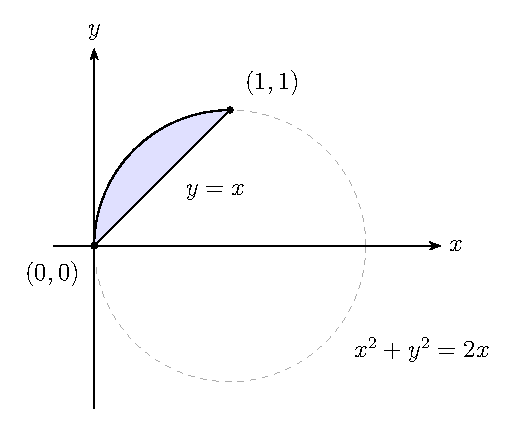
\includegraphics[width=\linewidth]{figures/q5-cartesian-to-polar.pdf}
\end{minipage}

\vfill
\begin{flushright}
\framebox(400,60){}
\end{flushright}

% Original cut-washer mass problem: retained left cap of 1 <= r <= 2.
\item
\begin{minipage}[t]{0.62\linewidth}
\raggedright
The shaded lamina is the part of $1\leq x^2+y^2\leq4$ with
\mbox{$-2\leq x\leq-1$}. Its density is $\delta(x,y)=x^2+y^2-1$.
Use polar coordinates to find its mass.

\medskip
\textit{Hint: First write the region's Cartesian bounds explicitly.
Then convert those bounds to polar coordinates. You may use}
\[
  \int\sec^4\theta\,d\theta
  =\tan\theta+\frac13\tan^3\theta+C.
\]
\end{minipage}\hfill
\begin{minipage}[t]{0.34\linewidth}
\vspace{0pt}
\centering
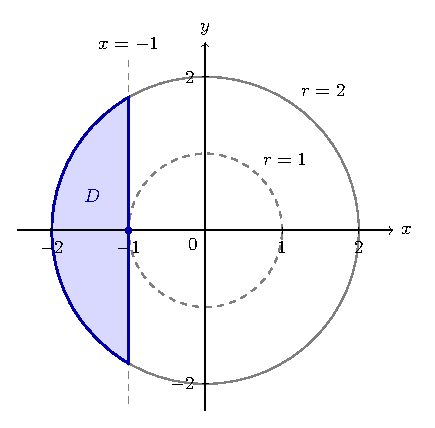
\includegraphics[width=\linewidth]{figures/q5-cut-washer.pdf}
\end{minipage}

\vfill
\begin{flushright}
\framebox(250,50){}
\end{flushright}

\newpage

% Adapted from BaohuaQ5Review.tex A2, with cone slope 2.
\item A solid has cylindrical bounds
\[
  \left\{
  \begin{aligned}
    &0\leq\theta\leq2\pi,\\
    &0\leq r\leq2,\\
    &r^2\leq z\leq2r.
  \end{aligned}
  \right.
\]
Sketch and shade its cross section in the entire $xz$-plane ($y=0$).
Label the points where the two boundary curves meet.

% Deliberately no answer box: the open space is for the final sketch.
\vfill

% Adapted from Moodle .009, P5-CE-V1, question 11721839: bounds only.
\item Write spherical-coordinate bounds for
\[
  E=\{(x,y,z):1\leq x^2+y^2+z^2\leq4,\ x\leq0,\ y\geq0\}.
\]
Here $\varphi$ is measured from the positive $z$-axis, and $\theta$ is the
azimuthal angle measured from the positive $x$-axis in the $xy$-plane.

\vfill
\begin{flushright}
\framebox(400,75){}
\end{flushright}

\end{enumerate}

\end{document}
